%\documentclass{article}
%\usepackage{graphicx,subfigure}
%\begin{document}

\begin{figure}[!h]
  \centering
  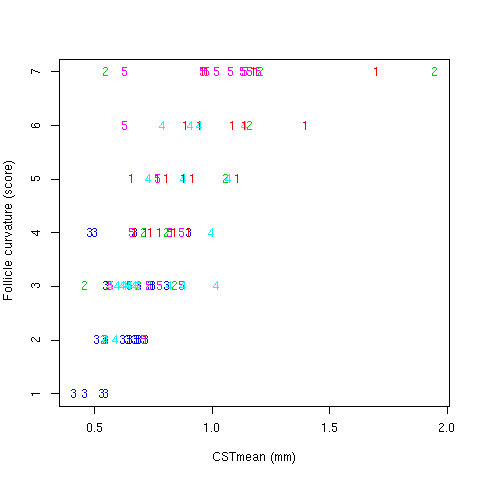
\includegraphics[width=1.0\textwidth]{CSTFc.png}
  \caption{Plot of CSTmean measurements against follicle curvature score. The numbered points reveal the Flock to which each data point belongs. The correlation of these points is 0.72 which is significant at the 1 percent level for 106 observations}
  \label{fig:CSTFc}
\end{figure}

%\end{document}

